%%%%%%%%%%%%%%%%%%%%%%%%%%%%%%%%%%%%%%%%%%%%%%%%%%%%%%%%%%%%%%%%%%%%%%%
%%%%%%%%%%%%%%%%%%%%%%%%%%%%%%%%%%%%%%%%%%%%%%%%%%%%%%%%%%%%%%%%%%%%%%%
%%%%%                                                                 %
%%%%%     <file_name>.tex                                             %
%%%%%                                                                 %
%%%%% Author:      <author>                                           %
%%%%% Created:     <date>                                             %
%%%%% Description: <description>                                      %
%%%%%                                                                 %
%%%%%%%%%%%%%%%%%%%%%%%%%%%%%%%%%%%%%%%%%%%%%%%%%%%%%%%%%%%%%%%%%%%%%%%
%%%%%%%%%%%%%%%%%%%%%%%%%%%%%%%%%%%%%%%%%%%%%%%%%%%%%%%%%%%%%%%%%%%%%%%

%%%%%%%%%%%%%%%%%%%%%%%%%%%%%%%%%%%%%%%%%%%%%%%%%%%%%%%%%%%%%%%%%%%%%%%
%%%%%                                                                 %
%%%%%     Document Class                                              %
%%%%%                                                                 %
%%%%%%%%%%%%%%%%%%%%%%%%%%%%%%%%%%%%%%%%%%%%%%%%%%%%%%%%%%%%%%%%%%%%%%%
\documentclass[%
 oneside,      % Use the same margins for odd and even pages (cannot
               % be used with the 'twoside' option). 
% twoside,      % Use different margins for odd and even pages (cannot
               % be used with the 'oneside' option).
 openany,      % Open chapters on odd and even pages.
 halfparskip,  % Create small spaces for new paragraphs but no indents.
]{scrbook}

%%%%%%%%%%%%%%%%%%%%%%%%%%%%%%%%%%%%%%%%%%%%%%%%%%%%%%%%%%%%%%%%%%%%%%%
%%%%%                                                                 %
%%%%%     Preamble                                                    %
%%%%%                                                                 %
%%%%%%%%%%%%%%%%%%%%%%%%%%%%%%%%%%%%%%%%%%%%%%%%%%%%%%%%%%%%%%%%%%%%%%%
% Load the preamble from another file.
%%%%%%%%%%%%%%%%%%%%%%%%%%%%%%%%%%%%%%%%%%%%%%%%%%%%%%%%%%%%%%%%%%%%%%%
%%%%%%%%%%%%%%%%%%%%%%%%%%%%%%%%%%%%%%%%%%%%%%%%%%%%%%%%%%%%%%%%%%%%%%%
%%%%%                                                                 %
%%%%%     preamble.tex                                                %
%%%%%                                                                 %
%%%%% Author:      Michael Muehlberghuber                             %
%%%%% Created:     01.07.2012                                         %
%%%%% Description: This file contains the preamble of the             %
%%%%%              Semester-/Master-Project LaTeX report example.     %
%%%%%                                                                 %
%%%%% History:                                                        %
%%%%%%%%%%%%%%                                                        %
%%%%% 2012/07/01:  *) Created initial version.                        %
%%%%%                                                                 %
%%%%%%%%%%%%%%%%%%%%%%%%%%%%%%%%%%%%%%%%%%%%%%%%%%%%%%%%%%%%%%%%%%%%%%%
%%%%%%%%%%%%%%%%%%%%%%%%%%%%%%%%%%%%%%%%%%%%%%%%%%%%%%%%%%%%%%%%%%%%%%%

%%%%%%%%%%%%%%%%%%%%%%%%%%%%%%%%%%%%%%%%%%%%%%%%%%%%%%%%%%%%%%%%%%%%%%%
%%%%%                                                                 %
%%%%%     Package Loading                                             %
%%%%%                                                                 %
%%%%%%%%%%%%%%%%%%%%%%%%%%%%%%%%%%%%%%%%%%%%%%%%%%%%%%%%%%%%%%%%%%%%%%%

% Determines the input encoding.
\usepackage[%
 utf8,
% latin1
]{inputenc}

% ---------------------------------------------------------------------

% Determines the output encoding.
\usepackage[T1]{fontenc}

% ---------------------------------------------------------------------

% Determines language settings.
\usepackage[%
 english    % You may change this to 'ngerman' in order to write a
            % german report.
]{babel}

% ---------------------------------------------------------------------

% Provides image loading.
\usepackage{graphicx}

% ---------------------------------------------------------------------

% Provides customization of chapter headings.
\usepackage[%
	Lenny     % Choose a nice layout for chapter headings.
]{fncychap}

% ---------------------------------------------------------------------

% Provides some blindtext.
\usepackage{lipsum}

% ---------------------------------------------------------------------

% Provides stretchable tables.
\usepackage{tabularx}

% ---------------------------------------------------------------------

% Provides some fancy boxes.
\usepackage{fancybox}

% ---------------------------------------------------------------------

% Provides subfigures.
\usepackage{subfig}

% ---------------------------------------------------------------------

% Provides colors in LaTeX.
\usepackage{xcolor}

% ---------------------------------------------------------------------

% Provides conditionals (for titlepage).
\usepackage{xifthen}

% ---------------------------------------------------------------------

% Provides the algorithm environment
\usepackage[ruled,%
            linesnumbered]{algorithm2e}

% ---------------------------------------------------------------------

% Provides bold greek math symbols.
\usepackage{bm}

% ---------------------------------------------------------------------

% Allows to include pdf documents.
\usepackage{pdfpages}

% ---------------------------------------------------------------------

% Provides nicer tables than the standard tables.
\usepackage{booktabs}

% ---------------------------------------------------------------------

% Provides simple line spacings.
\usepackage{setspace}

% ---------------------------------------------------------------------

% Provides simple line spacings.
\usepackage{geometry}
\geometry{
 a4paper,         % Paper size
 left=25mm,       % Left margin
 right=25mm,      % Right margin
 top=25mm,        % Top margin
 bottom=25mm      % Bottom margin
}

% ---------------------------------------------------------------------

% Provides more customizeable captions.
\usepackage{capt-of}

% ---------------------------------------------------------------------

% Provides small table of contents (e.g., for single chapters or the
% appendix).
\usepackage{minitoc}

% ---------------------------------------------------------------------

% Provides a simple command to describe a directory tree.
\usepackage{dirtree}

% ---------------------------------------------------------------------

%%%%%                                                             %%%%%
%%%%% ATTENTION: Loading further packagaes should go in here.     %%%%%
%%%%%                                                             %%%%%

% ---------------------------------------------------------------------

% Provides hyperlinks within your document. Should always be loaded at
% the end.
\usepackage{hyperref}

% ---------------------------------------------------------------------

% Provides multiple glossaries (incl. list acronyms, list of symbols,
% etc.).
\usepackage[%
 toc,              % Add the glossaries to the table of contents.
 acronym,          % Add a list of acronyms.
 section=chapter,  % Show glossary headers as chapters.
 nonumberlist,     % Do not print the page numbers next to glossary
                   % entries.
]{glossaries}

\usepackage{tikz}
\usetikzlibrary{shapes.geometric, arrows}


%%%%%%%%%%%%%%%%%%%%%%%%%%%%%%%%%%%%%%%%%%%%%%%%%%%%%%%%%%%%%%%%%%%%%%%
%%%%%                                                                 %
%%%%%     Custom Settings                                             %
%%%%%                                                                 %
%%%%%%%%%%%%%%%%%%%%%%%%%%%%%%%%%%%%%%%%%%%%%%%%%%%%%%%%%%%%%%%%%%%%%%%
% Do not use sans-serif fonts for all dispositions (chapters,
% sections, etc.)
\setkomafont{disposition}{\normalfont\bfseries}


%%%%%%%%%%%%%%%%%%%%%%%%%%%%%%%%%%%%%%%%%%%%%%%%%%%%%%%%%%%%%%%%%%%%%%%
%%%%%                                                                 %
%%%%%     Custom Macros                                               %
%%%%%                                                                 %
%%%%%%%%%%%%%%%%%%%%%%%%%%%%%%%%%%%%%%%%%%%%%%%%%%%%%%%%%%%%%%%%%%%%%%%
% Create an inline command for shell commands.
\newcommand{\shell}[1]{\texttt{#1}}

% Create an enviroment for a shell commands.
\newenvironment{shellenv}%
{\VerbatimEnvironment%
 \begin{Sbox}\begin{minipage}{0.97\textwidth}\begin{Verbatim}%
}%
{\end{Verbatim}\end{minipage}\end{Sbox}%
\setlength{\fboxsep}{6pt}\shadowbox{\TheSbox}}%

% Create an inline command for files.
\newcommand{\file}[1]{\texttt{#1}}

% Create a command for command parameters.
\newcommand{\parameter}[1]{$<$#1$>$}


%%%%%%%%%%%%%%%%%%%%%%%%%%%%%%%%%%%%%%%%%%%%%%%%%%%%%%%%%%%%%%%%%%%%%%%
%%%%%                                                                 %
%%%%%     Titlepage Macros - !!! DO NOT CHANGE !!!                    %
%%%%%                                                                 %
%%%%%%%%%%%%%%%%%%%%%%%%%%%%%%%%%%%%%%%%%%%%%%%%%%%%%%%%%%%%%%%%%%%%%%%
% Create a command for missing title page parameters.
\newcommand{\misspar}[1]{\textcolor{red}{\textbf{$<$#1$>$}}}

\makeatletter

% Redefine existing class macros as missing.
\title{\misspar{Specify Title}}%
\author{\misspar{Specify Author}}%
\date{\misspar{Specify Date}}%

% Define a command for setting the semester on the titlepage.
\def\@semester{\misspar{Specify Semester}}%
\newcommand{\setsemester}[1]{\def\@semester{#1}}%
\let\semester\setsemester%
\newcommand{\show@semester}{\@semester}%

% Define a command for setting the type of the report (Master Thesis,
% Semester Project, etc.) on the titlepage.
\def\@reporttype{\misspar{Specify Report Type}}%
\newcommand{\setreporttype}[1]{\def\@reporttype{#1}}%
\let\reporttype\setreporttype%
\newcommand{\show@reporttype}{\@reporttype}%

% Define a command for setting the image path for the image on the
% titlepage.
\def\@titlelogo{}%
\newcommand{\settitlelogo}[1]{\def\@titlelogo{#1}}%
\let\titlelogo\settitlelogo%

% Define a command for setting the image height on the titlepage.
\def\@logoheight{7cm}%
\newcommand{\setlogoheight}[1]{\def\@logoheight{#1}}%
\let\logoheight\setlogoheight%
\newcommand{\show@logoheight}{\@logoheight}%

% Define a command for setting the email on the titlepage.
\def\@email{\misspar{Specify E-Mail}}%
\newcommand{\setemail}[1]{\def\@email{#1}}%
\let\email\setemail%
\newcommand{\show@email}{\@email}%

% Define a command for setting the first supervisor on the titlepage.
\def\@firstsup{\misspar{Specify First Supervisor}}%
\newcommand{\setfirstsup}[1]{\def\@firstsup{#1}}%
\let\firstsup\setfirstsup%
\newcommand{\show@firstsup}{\@firstsup}%

% Define a command for setting the second supervisor on the titlepage.
\def\@secondsup{\misspar{Specify Second Supervisor}}%
\newcommand{\setsecondsup}[1]{\def\@secondsup{#1}}%
\let\secondsup\setsecondsup%
\newcommand{\show@secondsup}{\@secondsup}%

% Define a command for setting the professor on the titlepage.
\def\@professor{\misspar{Specify Professor}}%
\newcommand{\setprofessor}[1]{\def\@professor{#1}}%
\let\professor\setprofessor%
\newcommand{\show@professor}{\@professor}%

% Define a command for setting the margin on the title page.
\def\@titlepagemargin{3cm}%
\newcommand{\settitlepagemargin}[1]{\def\@titlepagemargin{#1}}%
\let\titlepagemargin\settitlepagemargin%
\newcommand{\show@titlepagemargin}{\@titlepagemargin}%

\makeatother


%%%%%
%%%%% Load the glossaries.
%%%%%
%%%%%%%%%%%%%%%%%%%%%%%%%%%%%%%%%%%%%%%%%%%%%%%%%%%%%%%%%%%%%%%%%%%%%%%
%%%%%                                                                 %
%%%%%     Make Glossaries                                             %
%%%%%                                                                 %
%%%%%%%%%%%%%%%%%%%%%%%%%%%%%%%%%%%%%%%%%%%%%%%%%%%%%%%%%%%%%%%%%%%%%%%

% Required to generate the index for the glossaries.
\makeglossaries

%%%%%%%%%%%%%%%%%%%%%%%%%%%%%%%%%%%%%%%%%%%%%%%%%%%%%%%%%%%%%%%%%%%%%%
%%%%%                                                                %
%%%%%     Definitions of all glossary entries which will appear in   %
%%%%%     the default (main) glossary.                               %
%%%%%                                                                %
%%%%%%%%%%%%%%%%%%%%%%%%%%%%%%%%%%%%%%%%%%%%%%%%%%%%%%%%%%%%%%%%%%%%%%

\newglossaryentry{monkey}{name=Monkey,description={Lorem ipsum dolor
sit amet, consetetur sadipscing elitr, sed diam nonumy eirmod tempor
invidunt ut labore et dolore magna aliquyam erat, sed diam
voluptua. At vero eos et accusam et justo duo dolores et ea
rebum. Stet clita kasd gubergren, no sea takimata sanctus est Lorem
ipsum dolor sit amet}}

\newglossaryentry{apple}{name=Apple,description={Lorem ipsum dolor sit
amet, consetetur sadipscing elitr, sed diam nonumy eirmod tempor
invidunt ut labore et dolore magna aliquyam erat, sed diam
voluptua. At vero eos et accusam et justo duo dolores et ea
rebum. Stet clita kasd gubergren, no sea takimata sanctus est Lorem
ipsum dolor sit amet}}

\newglossaryentry{guitar}{name=Guitar,description={Lorem ipsum dolor
sit amet, consetetur sadipscing elitr, sed diam nonumy eirmod tempor
invidunt ut labore et dolore magna aliquyam erat, sed diam
voluptua. At vero eos et accusam et justo duo dolores et ea
rebum. Stet clita kasd gubergren, no sea takimata sanctus est Lorem
ipsum dolor sit amet}}

\newglossaryentry{candle}{name=Candle,description={Lorem ipsum dolor
sit amet, consetetur sadipscing elitr, sed diam nonumy eirmod tempor
invidunt ut labore et dolore magna aliquyam erat, sed diam
voluptua. At vero eos et accusam et justo duo dolores et ea
rebum. Stet clita kasd gubergren, no sea takimata sanctus est Lorem
ipsum dolor sit amet}}

\newglossaryentry{snake}{name=Snake,description={Lorem ipsum dolor
sit amet, consetetur sadipscing elitr, sed diam nonumy eirmod tempor
invidunt ut labore et dolore magna aliquyam erat, sed diam
voluptua. At vero eos et accusam et justo duo dolores et ea
rebum. Stet clita kasd gubergren, no sea takimata sanctus est Lorem
ipsum dolor sit amet}}


% Add all glossary entries to the glossary, even if they have not been
% referenced.
\glsaddall[types={main}]


%%%%%%%%%%%%%%%%%%%%%%%%%%%%%%%%%%%%%%%%%%%%%%%%%%%%%%%%%%%%%%%%%%%%%%
%%%%%                                                                %
%%%%%     Definitions of all acronyms which will appear in the list  %
%%%%%     of acronyms.                                               %
%%%%%                                                                %
%%%%%%%%%%%%%%%%%%%%%%%%%%%%%%%%%%%%%%%%%%%%%%%%%%%%%%%%%%%%%%%%%%%%%%

\newacronym{iis}{IIS}{Integrated Systems Laboratory}
\newacronym{asic}{ASIC}{Application-Specific Integrated Circuit}
\newacronym{fpga}{FPGA}{Field Programmable Gate Array}
\newacronym{led}{LED}{Light-Emitting Diode}
\newacronym{nist}{NIST}{National Institute of Standards and
Technology}
\newacronym{aes}{AES}{Advanced Encryption Standard}
\newacronym{ecc}{ECC}{Elliptic Curve Cryptography}
\newacronym{ecdsa}{ECDSA}{Elliptic Curve Digital Signature Algorithm}
\newacronym{des}{DES}{Data Encryption Standard}
\newacronym{wysiwyg}{WYSIWYG}{What You See Is What You Get}
\newacronym{pdf}{PDF}{Portable Document Format}
\newacronym{eps}{EPS}{Encapsulated PostScript}
\newacronym{dvi}{DVI}{Device Independent File Format }
\newacronym{ic}{IC}{Integrated Circuit}

\newacronym{wdt}{WDT}{Watchdog Timer}

% Add all acronyms to the list of acronyms even if they have not been
% referenced.
\glsaddall[types={\acronymtype}]


% Define which source files should actually been processed.
%\includeonly{./content/06-design_implementation}


%%%%%%%%%%%%%%%%%%%%%%%%%%%%%%%%%%%%%%%%%%%%%%%%%%%%%%%%%%%%%%%%%%%%%%%
%%%%%                                                                 %
%%%%%     Document Settings                                           %
%%%%%                                                                 %
%%%%%%%%%%%%%%%%%%%%%%%%%%%%%%%%%%%%%%%%%%%%%%%%%%%%%%%%%%%%%%%%%%%%%%%

%%%%% Mandatory title page settings.
\title{Ensuring Fault Tolerance in the CROC SoC: A Hardware-Centric Approach to Watchdog Timer Implementation}
\author{Miguel Correa and Elio Wanner}
\email{corream@ethz.ch, ewanner@ethz.ch}
\date{\today}
\semester{Spring Semester 2025}
\reporttype{VLSI 2 Course Project}
%\firstsup{Title A, Title B John Doe, john@doe.com}
%\secondsup{Title C, Title D Jane Doe, jane@doe.com}
\professor{Frank Kagan Gürkaynak, kgf@iis.ee.ethz.ch}

%%%%% Optional title page settings.
\titlelogo{./figures/titlepage_logo}  % Title page logo path.
\logoheight{7cm}                      % Height of the title page logo.
\titlepagemargin{3cm}                 % Margin on the title page.


%%%%%%%%%%%%%%%%%%%%%%%%%%%%%%%%%%%%%%%%%%%%%%%%%%%%%%%%%%%%%%%%%%%%%%%
%%%%%                                                                 %
%%%%%     Start of Document                                           %
%%%%%                                                                 %
%%%%%%%%%%%%%%%%%%%%%%%%%%%%%%%%%%%%%%%%%%%%%%%%%%%%%%%%%%%%%%%%%%%%%%%
\begin{document}

% Prepare document for minitoc insertions.
\dominitoc

\frontmatter

% Create title.
%%%%%%%%%%%%%%%%%%%%%%%%%%%%%%%%%%%%%%%%%%%%%%%%%%%%%%%%%%%%%%%%%%%%%%%
%%%%%%%%%%%%%%%%%%%%%%%%%%%%%%%%%%%%%%%%%%%%%%%%%%%%%%%%%%%%%%%%%%%%%%%
%%%%%                                                                 %
%%%%%     <file_name>.tex                                             %
%%%%%                                                                 %
%%%%% Author:      <author>                                           %
%%%%% Created:     <date>                                             %
%%%%% Description: <description>                                      %
%%%%%                                                                 %
%%%%%%%%%%%%%%%%%%%%%%%%%%%%%%%%%%%%%%%%%%%%%%%%%%%%%%%%%%%%%%%%%%%%%%%
%%%%%%%%%%%%%%%%%%%%%%%%%%%%%%%%%%%%%%%%%%%%%%%%%%%%%%%%%%%%%%%%%%%%%%%
\makeatletter
\newgeometry{margin = \@titlepagemargin}
\begin{titlepage}

 % Remove the page number in the footer.
 \thispagestyle{empty}

 \begin{center}
  \begin{minipage}[b]{0.45\linewidth}
   \vspace{0pt}	
   
\includegraphics[width=0.8\linewidth]{./figures/eth_logo}
  \end{minipage}\hfill
  \begin{minipage}{0.45\textwidth}
%   \vspace{-1cm}\flushright{Institut f\"ur Integrierte Systeme\\Integrated Systems Laboratory}
   \vspace{-0.55cm}\flushright{\fontfamily{let}\fontseries{b}\fontsize{\@xpt}{18}\selectfont Institut f\"ur Integrierte Systeme\\Integrated Systems Laboratory}
  \end{minipage}

  \vspace{0.1cm}

  \hspace*{0.15cm}\rule{0.985\textwidth}{0.4pt}

  \vspace{0.5cm}

  {\Large\textsc{Department of Information Technology and \\Electrical Engineering}}

  \vspace{0.2cm}

  \show@semester

  \vfill

  \begin{spacing}{2.0}
  {\Huge\textbf{\@title}}
  \end{spacing}

  \vspace{0.2cm}

  \show@reporttype

  \vfill
  
  \ifx\@titlelogo\@empty
   \relax
  \else
   \includegraphics[height = \@logoheight]{\@titlelogo}
  \fi
    
  \vfill

  {\Large \@author}\\
  {\@email}
  
  \vfill
  
  \@date

  \vfill
  
  \begin{tabular}{ll}
   %Supervisors: & \show@firstsup \\
   %             & \show@secondsup \\
   \rule{0pt}{3ex}Professor: & \show@professor \\
  \end{tabular}

 \end{center}
\end{titlepage}
\restoregeometry
\makeatother

%\maketitle

% Include acknowledgements, abstract, etc...
%%%%%%%%%%%%%%%%%%%%%%%%%%%%%%%%%%%%%%%%%%%%%%%%%%%%%%%%%%%%%%%%%%%%%%%
%%%%%%%%%%%%%%%%%%%%%%%%%%%%%%%%%%%%%%%%%%%%%%%%%%%%%%%%%%%%%%%%%%%%%%%
%%%%%                                                                 %
%%%%%     <file_name>.tex                                             %
%%%%%                                                                 %
%%%%% Author:      <author>                                           %
%%%%% Created:     <date>                                             %
%%%%% Description: <description>                                      %
%%%%%                                                                 %
%%%%%%%%%%%%%%%%%%%%%%%%%%%%%%%%%%%%%%%%%%%%%%%%%%%%%%%%%%%%%%%%%%%%%%%
%%%%%%%%%%%%%%%%%%%%%%%%%%%%%%%%%%%%%%%%%%%%%%%%%%%%%%%%%%%%%%%%%%%%%%%

\chapter*{Abstract}
This report summarizes the work done in the VLSI 2 course project. 
The project consisted of extending the Croc SoC with a Watchdog Timer. 

% Insert table of contents, list of figures, and list of tables.
\tableofcontents
%\listoffigures
%\listoftables

% Print list of acronyms.
% \setlength{\glslistdottedwidth}{0.2\linewidth}
% \printglossary[type=\acronymtype,style=listdotted,title=List of Acronyms]


%%%%%
%%%%% Start the actual main content part.
%%%%%
\mainmatter

% Include the actual content files.
%%%%%%%%%%%%%%%%%%%%%%%%%%%%%%%%%%%%%%%%%%%%%%%%%%%%%%%%%%%%%%%%%%%%%%%
%%%%%%%%%%%%%%%%%%%%%%%%%%%%%%%%%%%%%%%%%%%%%%%%%%%%%%%%%%%%%%%%%%%%%%%
%%%%%                                                                 %
%%%%%     01_introduction.tex                                         %
%%%%%                                                                 %
%%%%% Author:      Miguel Correa, Elio Warner                         %
%%%%% Created:     22.03.2024                                         %
%%%%% Description: - Overview of the Croc SoC and its open-source     %
%%%%%                nature                                           %
%%%%%              - Why a watchdog timer (WDT) was needed            %   
%%%%%              - Goals and expected improvements                  %
%%%%%                                                                 %
%%%%%%%%%%%%%%%%%%%%%%%%%%%%%%%%%%%%%%%%%%%%%%%%%%%%%%%%%%%%%%%%%%%%%%%
%%%%%%%%%%%%%%%%%%%%%%%%%%%%%%%%%%%%%%%%%%%%%%%%%%%%%%%%%%%%%%%%%%%%%%%

\chapter{Introduction}
\label{chap:introduction}

\section{Overview of the Croc SoC and its open-source nature}
\begin{itemize}
  \item{Picture of Croc SoC}
  \item{Quick explanation of its main parts and mostly what we are using ==> user_domain}
  \item{Mention that it is open-source and the importance of this, but also why it has to be robust for it to be competitive with closed source in real life scenarios}
\end{itemize}
\section{Why a watchdog timer (WDT) was needed}
\begin{itemize}
  \item Real life scenario as an example of anoying stuck in a loop chip (if possible, true historic reference)
  \item Explain what is a watchdog timer and how it would prevent this
  \item From this go on and conclude it was needed on the Croc SoC
\end{itemize}

\section{Goals and expected improvements}
\begin{itemize}
  \item Emphasize on the main goals of the watchdog, with bullet points if possible to emphasize even more. THe main goals being: improve robustness while keeping area and throughput as low as possible. (should we add more goals?)
\end{itemize}

%%% Local Variables: 
%%% mode: latex
%%% TeX-master: "../report_template"
%%% End: 

%%%%%%%%%%%%%%%%%%%%%%%%%%%%%%%%%%%%%%%%%%%%%%%%%%%%%%%%%%%%%%%%%%%%%%%
%%%%%%%%%%%%%%%%%%%%%%%%%%%%%%%%%%%%%%%%%%%%%%%%%%%%%%%%%%%%%%%%%%%%%%%
%%%%%                                                                 %
%%%%%     02_related_work.tex                                         %
%%%%%                                                                 %
%%%%% Author:      Miguel Correa, Elio Warner                         %
%%%%% Created:     22.03.2024                                         %
%%%%% Description: - Overview of existing watchdog timer              %
%%%%%                implementation                                   %
%%%%%              - Justification for our approach                   %
%%%%%                                                                 %
%%%%%%%%%%%%%%%%%%%%%%%%%%%%%%%%%%%%%%%%%%%%%%%%%%%%%%%%%%%%%%%%%%%%%%%
%%%%%%%%%%%%%%%%%%%%%%%%%%%%%%%%%%%%%%%%%%%%%%%%%%%%%%%%%%%%%%%%%%%%%%%

\chapter{Related Works}
\label{chap:related_work}

\section{Overview of existing watchdog timer implementation}
\begin{itemize}
  \item State several possible watchdog implementations, with sources.
  \item Explain that it is possible to keep it really simple or to complicate
    it by adding some features, like having a log to know why the watchdog triggered.
\end{itemize}

\section{Justification for our approach}
Now, explain our choice to keep it small, simple, energy efficient easy to understand
and easy to "take over" if it is needed for something else.
Explain that the trade off gains in robustness of croc vs complication of watch dog is
the best by keeping the watchdog simple.

%%%%%%%%%%%%%%%%%%%%%%%%%%%%%%%%%%%%%%%%%%%%%%%%%%%%%%%%%%%%%%%%%%%%%%%
%%%%%%%%%%%%%%%%%%%%%%%%%%%%%%%%%%%%%%%%%%%%%%%%%%%%%%%%%%%%%%%%%%%%%%%
%%%%%                                                                 %
%%%%%     03_methodology.tex                                          %
%%%%%                                                                 %
%%%%% Author:      Miguel Correa, Elio Warner                         %
%%%%% Created:     22.03.2024                                         %
%%%%% Description: - Design choices for WDT                           %
%%%%%                (e.g., countdown vs. count-up, reset duration)   %
%%%%%              - Testing strategy (testbenches, simulation tools) %
%%%%%              - Debugging and iteration process                  %
%%%%%                                                                 %
%%%%%%%%%%%%%%%%%%%%%%%%%%%%%%%%%%%%%%%%%%%%%%%%%%%%%%%%%%%%%%%%%%%%%%%
%%%%%%%%%%%%%%%%%%%%%%%%%%%%%%%%%%%%%%%%%%%%%%%%%%%%%%%%%%%%%%%%%%%%%%%


\chapter{Methodology}
\label{chap:methodology}

\section{Design choices for WDT (e.g., countdown vs. count-up, reset duration)}
Explain that we decided to make a simple watchdog, independent from croc to keep it simple.
Then, we added a wrapper to be able to connect it to OBI and croc.
Our watchdog uses cout-up (was our own choice) and have a 1 cycle reset duration, 
wich we found enough.

\section{Testing strategy (testbenches, simulation tools)}
At each step we tested our watchdog, from the simple watchdog to the communication with obi and finally the whole connected croc.
If we have time, we want to test a real life scenario (maybe a gpio that returns nothing so our program is stuck?).

\section{Debugging and iteration process}
By separating the work in easy, well separated steps it was easy to debbug.


%%%%%%%%%%%%%%%%%%%%%%%%%%%%%%%%%%%%%%%%%%%%%%%%%%%%%%%%%%%%%%%%%%%%%%%
%%%%%%%%%%%%%%%%%%%%%%%%%%%%%%%%%%%%%%%%%%%%%%%%%%%%%%%%%%%%%%%%%%%%%%%
%%%%%                                                                 %
%%%%%     04_wdt_implementation.tex                                   %
%%%%%                                                                 %
%%%%% Author:      Miguel Correa, Elio Wanner                         %
%%%%% Created:     17.03.2025                                         %
%%%%% Description: In here is the description of the hardware         %
%%%%%                                                                 %
%%%%%%%%%%%%%%%%%%%%%%%%%%%%%%%%%%%%%%%%%%%%%%%%%%%%%%%%%%%%%%%%%%%%%%%
%%%%%%%%%%%%%%%%%%%%%%%%%%%%%%%%%%%%%%%%%%%%%%%%%%%%%%%%%%%%%%%%%%%%%%%

\chapter{Hardware Architecture}
This chapter describes the hardware architecture of the Watchdog Timer that we implemented in the Croc SoC.
In the different sections we talk about different implementations with different features and complexities.

\section{Simple Watchdog Timer}
\subsection{Hardware implementation}
The first implementation of the Watchdog Timer is the simplest one we could imagine. 
As shown in Figure \ref{fig:simple_WDT}, the WDT is composed of
very few components. The main component is the counter, which is
incremented every clock cycle and implemented as a flip-flop. The counter is connected to a comparator
that checks if the counter has reached a certain value. If the counter
reaches the value, the comparator will trigger a reset signal that will
reset the system. Otherwise, we keep incrementing the counter. As soon as we get
a kick signal, the counter is reset to zero.

\begin{figure}[h]
\centering
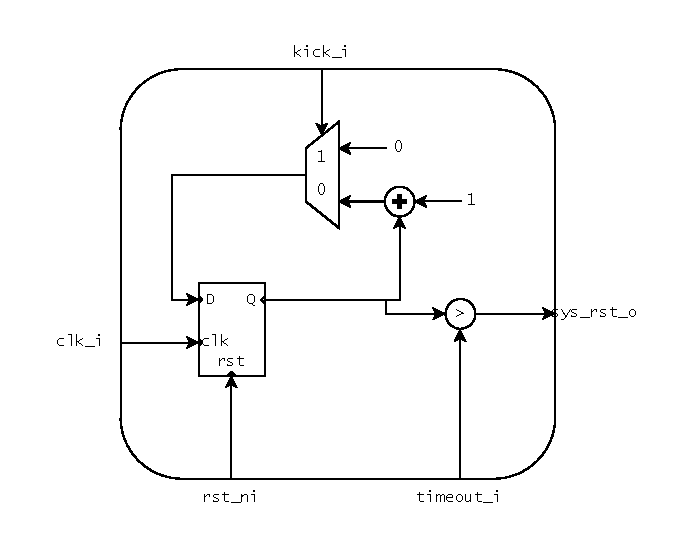
\includegraphics[width=0.7\textwidth]{./figures/simple_WDT}
\caption{Simple Watchdog Timer Architecture}
\label{fig:simple_WDT}
\end{figure}

\subsection{Tests and Results}
Explain how we did the tests (python files to generate stimuli + expected then compare), show figure.
Explain that the results were always good at the end.

\subsection{Conclusion}
Explain that thanks to our approach we found that the watchdog works fine, so if a future problem would come it would come from the wrapper.

\section{Watchdog Wrapper}
\subsection{Hardware implementation}
Add a graph of the watchdog wrapper, and maybe a figure of how it connects to the OBI protocol.

\subsection{Tests and Results}
We checked the functionality of our wrapper by running a helloword.c wich sets the timeout value and sends periodic kicks befor getting stuck in an impossible task. Our watchdog was successfully set thanks to the correctness of the wrapper and it allowed us to reset the program. We also checked the VCD to see if we could find any anormalities, but our wrapper respects OBI protocol :) .

%%%%%%%%%%%%%%%%%%%%%%%%%%%%%%%%%%%%%%%%%%%%%%%%%%%%%%%%%%%%%%%%%%%%%%%
%%%%%%%%%%%%%%%%%%%%%%%%%%%%%%%%%%%%%%%%%%%%%%%%%%%%%%%%%%%%%%%%%%%%%%%
%%%%%                                                                 %
%%%%%     05_evaluation.tex                                           %
%%%%%                                                                 %
%%%%% Author:      Miguel Correa, Elio Warner                         %
%%%%% Created:     22.03.2024                                         %
%%%%% Description: - Simulation results for v1 and v2                 %
%%%%%              - Performance comparison (goal achieved?)          %
%%%%%              - Trade-offs between versions                      %
%%%%%                                                                 %
%%%%%%%%%%%%%%%%%%%%%%%%%%%%%%%%%%%%%%%%%%%%%%%%%%%%%%%%%%%%%%%%%%%%%%%
%%%%%%%%%%%%%%%%%%%%%%%%%%%%%%%%%%%%%%%%%%%%%%%%%%%%%%%%%%%%%%%%%%%%%%%


\chapter{Evaluation}

\section{Simulation results for v1 and v2}

\section{Performance comparison (goal achieved?)}

\section{Trade-offs between versions}

%%%%%%%%%%%%%%%%%%%%%%%%%%%%%%%%%%%%%%%%%%%%%%%%%%%%%%%%%%%%%%%%%%%%%%%%
%%%%%%%%%%%%%%%%%%%%%%%%%%%%%%%%%%%%%%%%%%%%%%%%%%%%%%%%%%%%%%%%%%%%%%%
%%%%%                                                                 %
%%%%%     06_discussion.tex                                           %
%%%%%                                                                 %
%%%%% Author:      Miguel Correa, Elio Warner                         %
%%%%% Created:     22.03.2024                                         %
%%%%% Description: - Strengths and limitations of each approach       %
%%%%%              - Potential improvements (e.g., three-stage WDT)   %
%%%%%              - Lessons learned from the implementation          %
%%%%%                                                                 %
%%%%%%%%%%%%%%%%%%%%%%%%%%%%%%%%%%%%%%%%%%%%%%%%%%%%%%%%%%%%%%%%%%%%%%%
%%%%%%%%%%%%%%%%%%%%%%%%%%%%%%%%%%%%%%%%%%%%%%%%%%%%%%%%%%%%%%%%%%%%%%%

\chapter{Discussion}
\label{chap:discussion}

\section{Strengths and limitations of each approach}

\section{Potential improvements (e.g., three-stage WDT)}

\section{Lessons learned from the implementation}
%%%%%%%%%%%%%%%%%%%%%%%%%%%%%%%%%%%%%%%%%%%%%%%%%%%%%%%%%%%%%%%%%%%%%%%
%%%%%%%%%%%%%%%%%%%%%%%%%%%%%%%%%%%%%%%%%%%%%%%%%%%%%%%%%%%%%%%%%%%%%%%
%%%%%                                                                 %
%%%%%     07_conclusion.tex                                           %
%%%%%                                                                 %
%%%%% Author:      Miguel Correa, Elio Warner                         %
%%%%% Created:     22.03.2024                                         %
%%%%% Description: - Summary of key findings                          %    
%%%%%              - Future work and next steps                       %
%%%%%                                                                 %
%%%%%%%%%%%%%%%%%%%%%%%%%%%%%%%%%%%%%%%%%%%%%%%%%%%%%%%%%%%%%%%%%%%%%%%
%%%%%%%%%%%%%%%%%%%%%%%%%%%%%%%%%%%%%%%%%%%%%%%%%%%%%%%%%%%%%%%%%%%%%%%

\chapter{Conclusion}
\label{chap:conclusion}

\section{Summary of key findings}

\section{Future work and next steps}


%%%%%
%%%%% Start of additional parts.
%%%%%
\appendix

\backmatter

% Print the main glossary.
% \printglossary[type=main,title=Glossary]


% Print the bibliography.
\nocite*{} % Print non-cited references as well.
% \bibliographystyle{IEEEtran}
% \bibliography{IEEEabrv,./bib/main}


\end{document}
%%%%%%%%%%%%%%%%%%%%%%%%%%%%%%%%%%%%%%%%%%%%%%%%%%%%%%%%%%%%%%%%%%%%%%%
%%%%%                                                                 %
%%%%%     End of Document                                             %
%%%%%                                                                 %
%%%%%%%%%%%%%%%%%%%%%%%%%%%%%%%%%%%%%%%%%%%%%%%%%%%%%%%%%%%%%%%%%%%%%%%
